\documentclass[11pt,twocolumn,letterpaper]{article}
\usepackage[english]{babel}
\usepackage[utf8x]{inputenc}
\usepackage[T1]{fontenc}
\usepackage[font=small,skip=0pt]{caption}
\captionsetup[figure]{font=small,skip=0pt}
\usepackage[a4paper,top=2cm,bottom=2cm,left=2cm,right=2cm,marginparwidth=1.75cm]{geometry}
\usepackage{setspace}
\usepackage{amsmath}
\usepackage{graphicx}
\setlength {\marginparwidth}{2cm}
\usepackage[colorinlistoftodos]{todonotes}
\usepackage[colorlinks=true, allcolors=blue]{hyperref}
\usepackage{natbib}
\usepackage{siunitx}
%% Title
\title{
		\usefont{OT1}{bch}{b}{n}
		\normalfont \normalsize \textsc{University of Toronto Engineering Science CIV 102} \\ [11pt]
		\huge Bridge Project  \\
        
\selectlanguage{english}
\author{Group 701: Ivy Tan, Tyler Tian, Julia Ye (TA: Laurence Yin)}
\date{\today}
}

\begin{document}
\singlespacing
\maketitle

\section*{Introduction}
Our group analyzed how Design 0 would perform under train load and 200N point loads. We optimized Design 0 by adding or removing features to counteract the predicted failure causes. The final design was reached through rounds of iterations. This report will present our analysis on Design 0 and optimized design, justify the improvements and explain our construction process.

\section*{Design 0}
\vspace{-1em}
\begin{table}[h]
\begin{center}
\begin{tabular}{|cc|} 
\hline
\multicolumn{1}{|c}{} & \multicolumn{1}{c|}{Value} \\
\hline
$\Bar{y}$ &   $41.7\si{mm}$ \\
$A$ &   $438\si{mm^2}$ \\
$I$ &   $416000\si{mm^4}$ \\
$Q$ &   $6250\si{mm^3}$ \\
\hline
\end{tabular}
\caption{Cross Section Properties}
\end{center}
\end{table}
\begin{figure}[h]
  \centering
    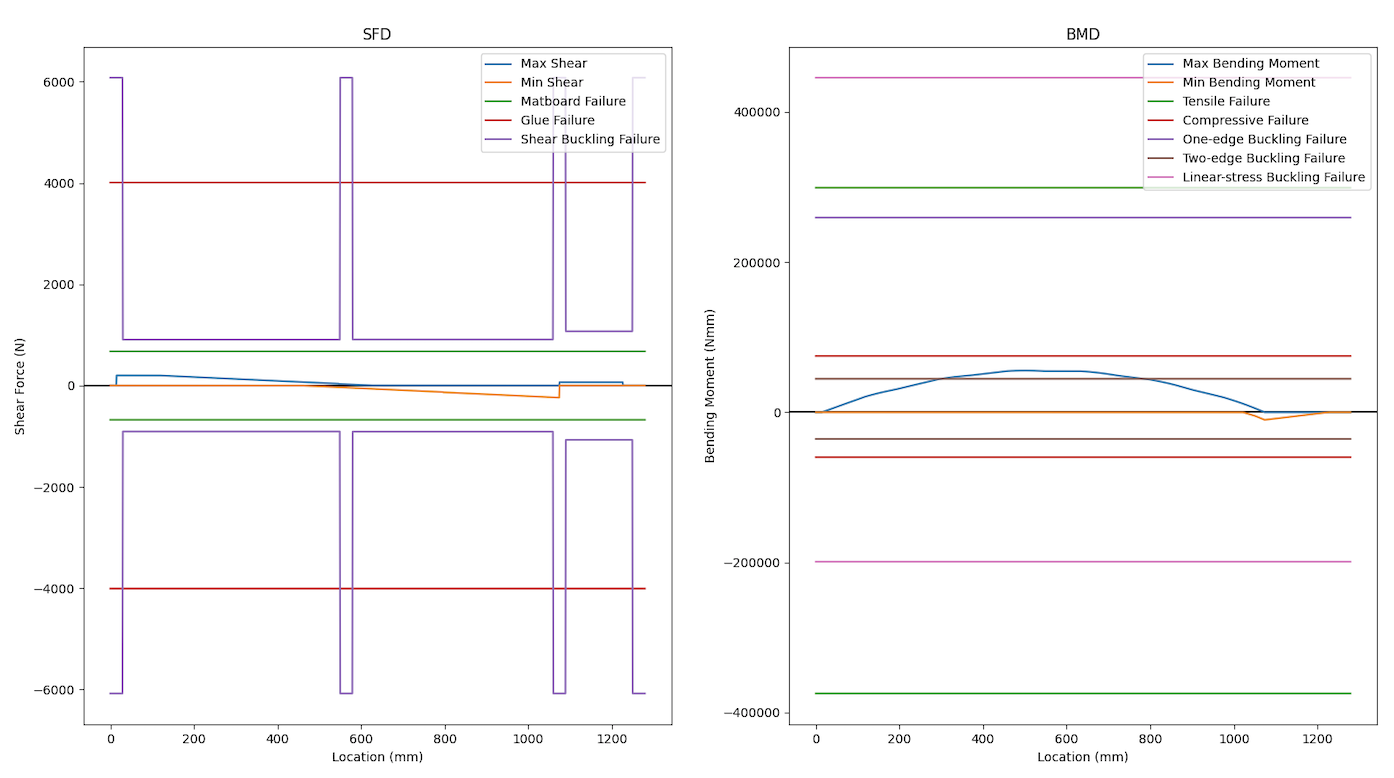
\includegraphics[width=.4\textwidth]{figures/S,BTrainFailure.png}
    \caption {Train Load at Failure (Design 0)}
    \label{fig:design0_train}
  \hfill
\end{figure}

\subsection*{Train Load}
Design 0 fails by local buckling of the middle top flange (two-edge buckling) (Figure \ref{fig:design0_train}). 
\begin{table}[h]
\begin{center}
\begin{tabular}{|cc|} 
\hline
\multicolumn{1}{|c}{FOS} & \multicolumn{1}{c|}{Value} \\
\hline
Shear &   $2.84$ \\
Bending Moment &   $0.802$ \\
\hline
\end{tabular}
\caption{Factor of Safety}
\end{center}
\end{table}
\begin{figure}[h!]
  \centering
    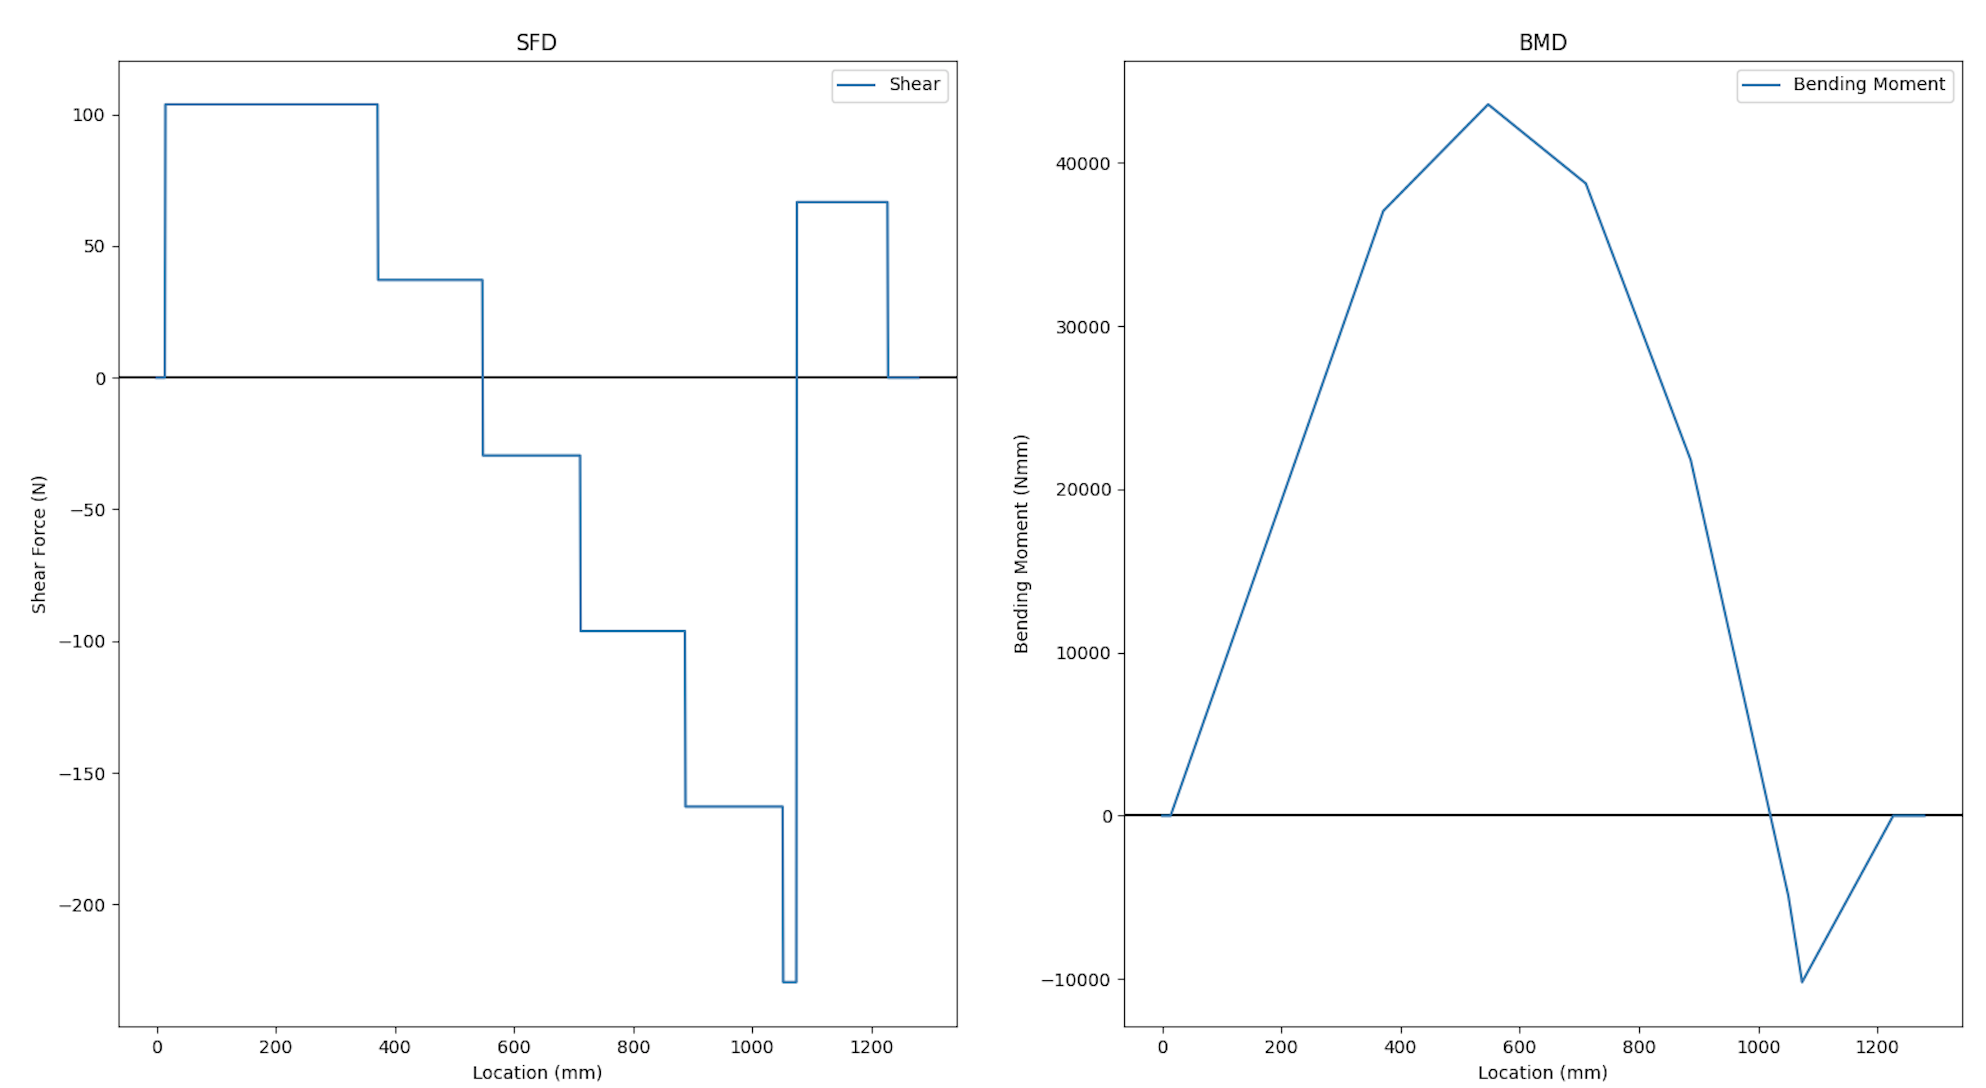
\includegraphics[width=.39\textwidth]{figures/S,BTrainatend.png}
    \caption {Train load at the end of the bridge}
  \hfill
\end{figure}
\begin{figure}[h!]
  \centering
    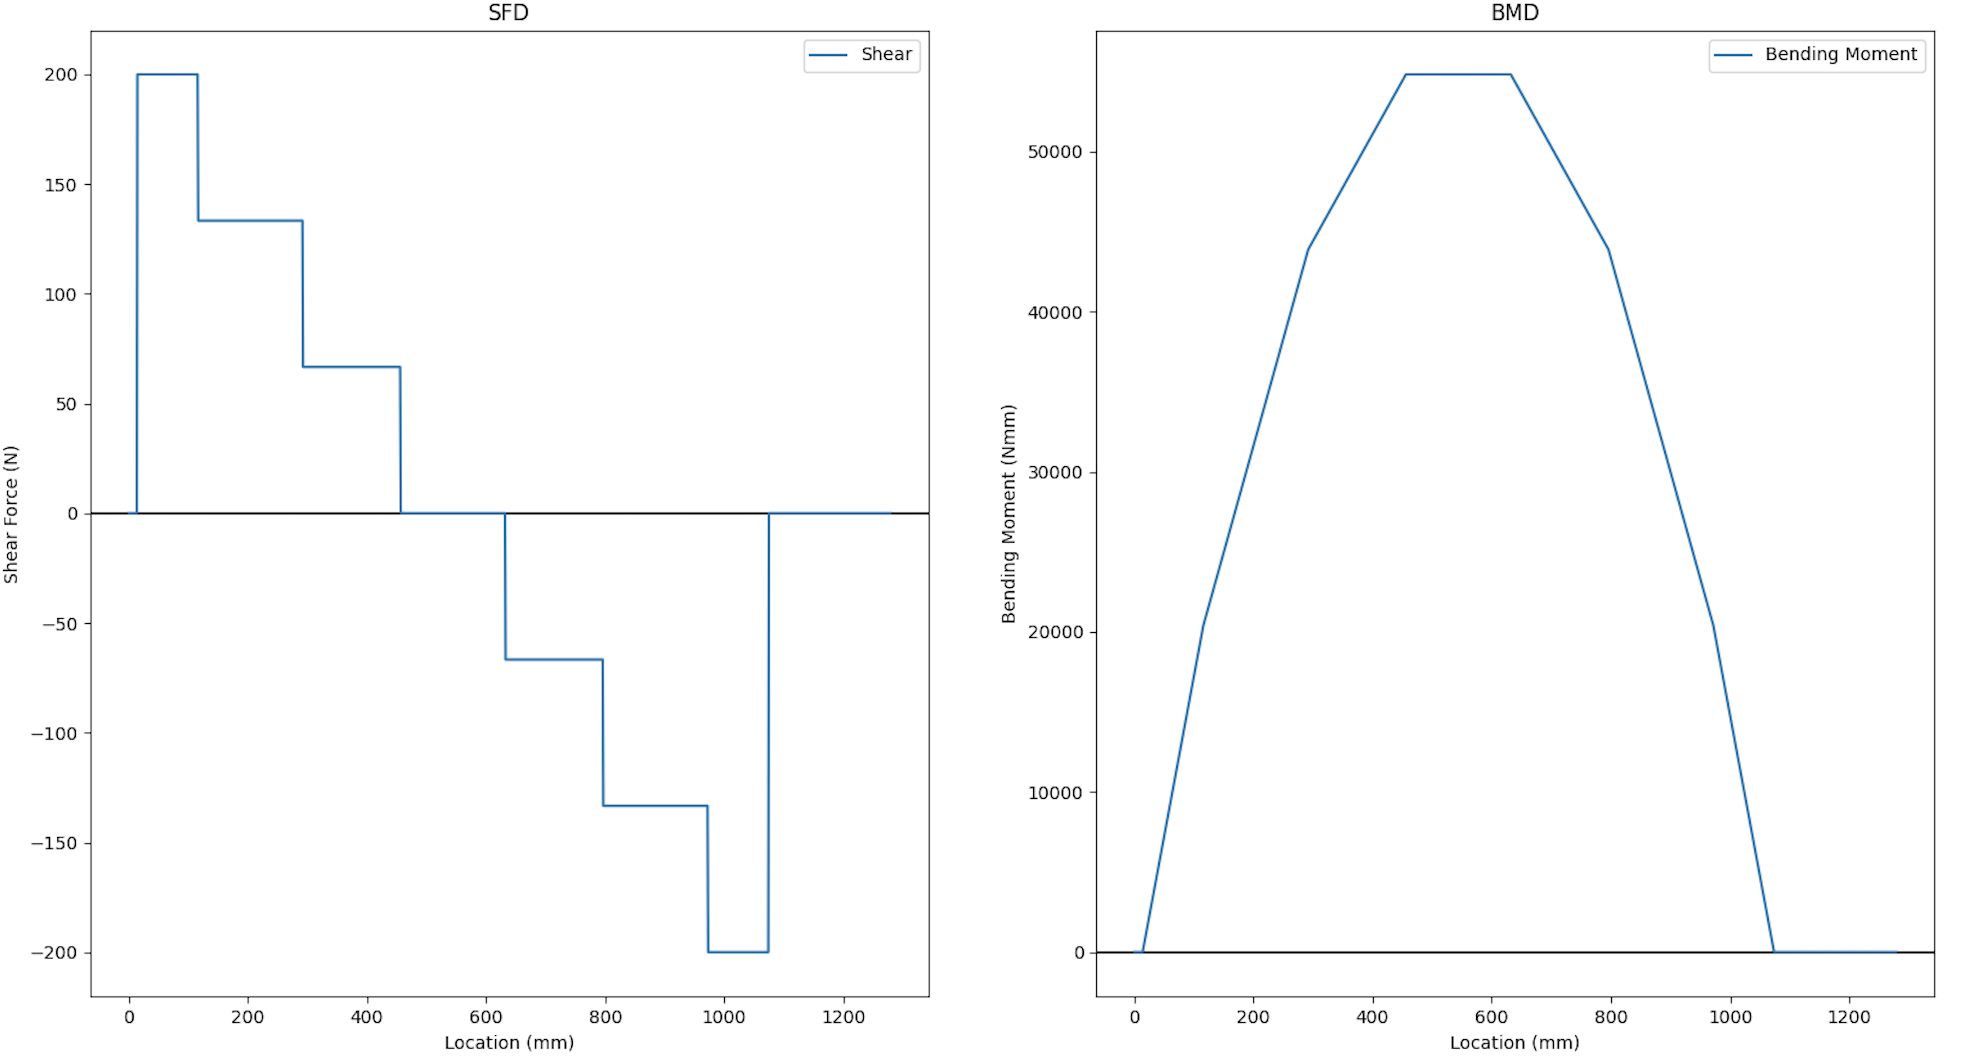
\includegraphics[width=.39\textwidth]{figures/S,BTrainmiddle.png}
    \caption {Train load in the middle of the bridge}
  \hfill
\end{figure}
\begin{figure}[h!]
  \centering
    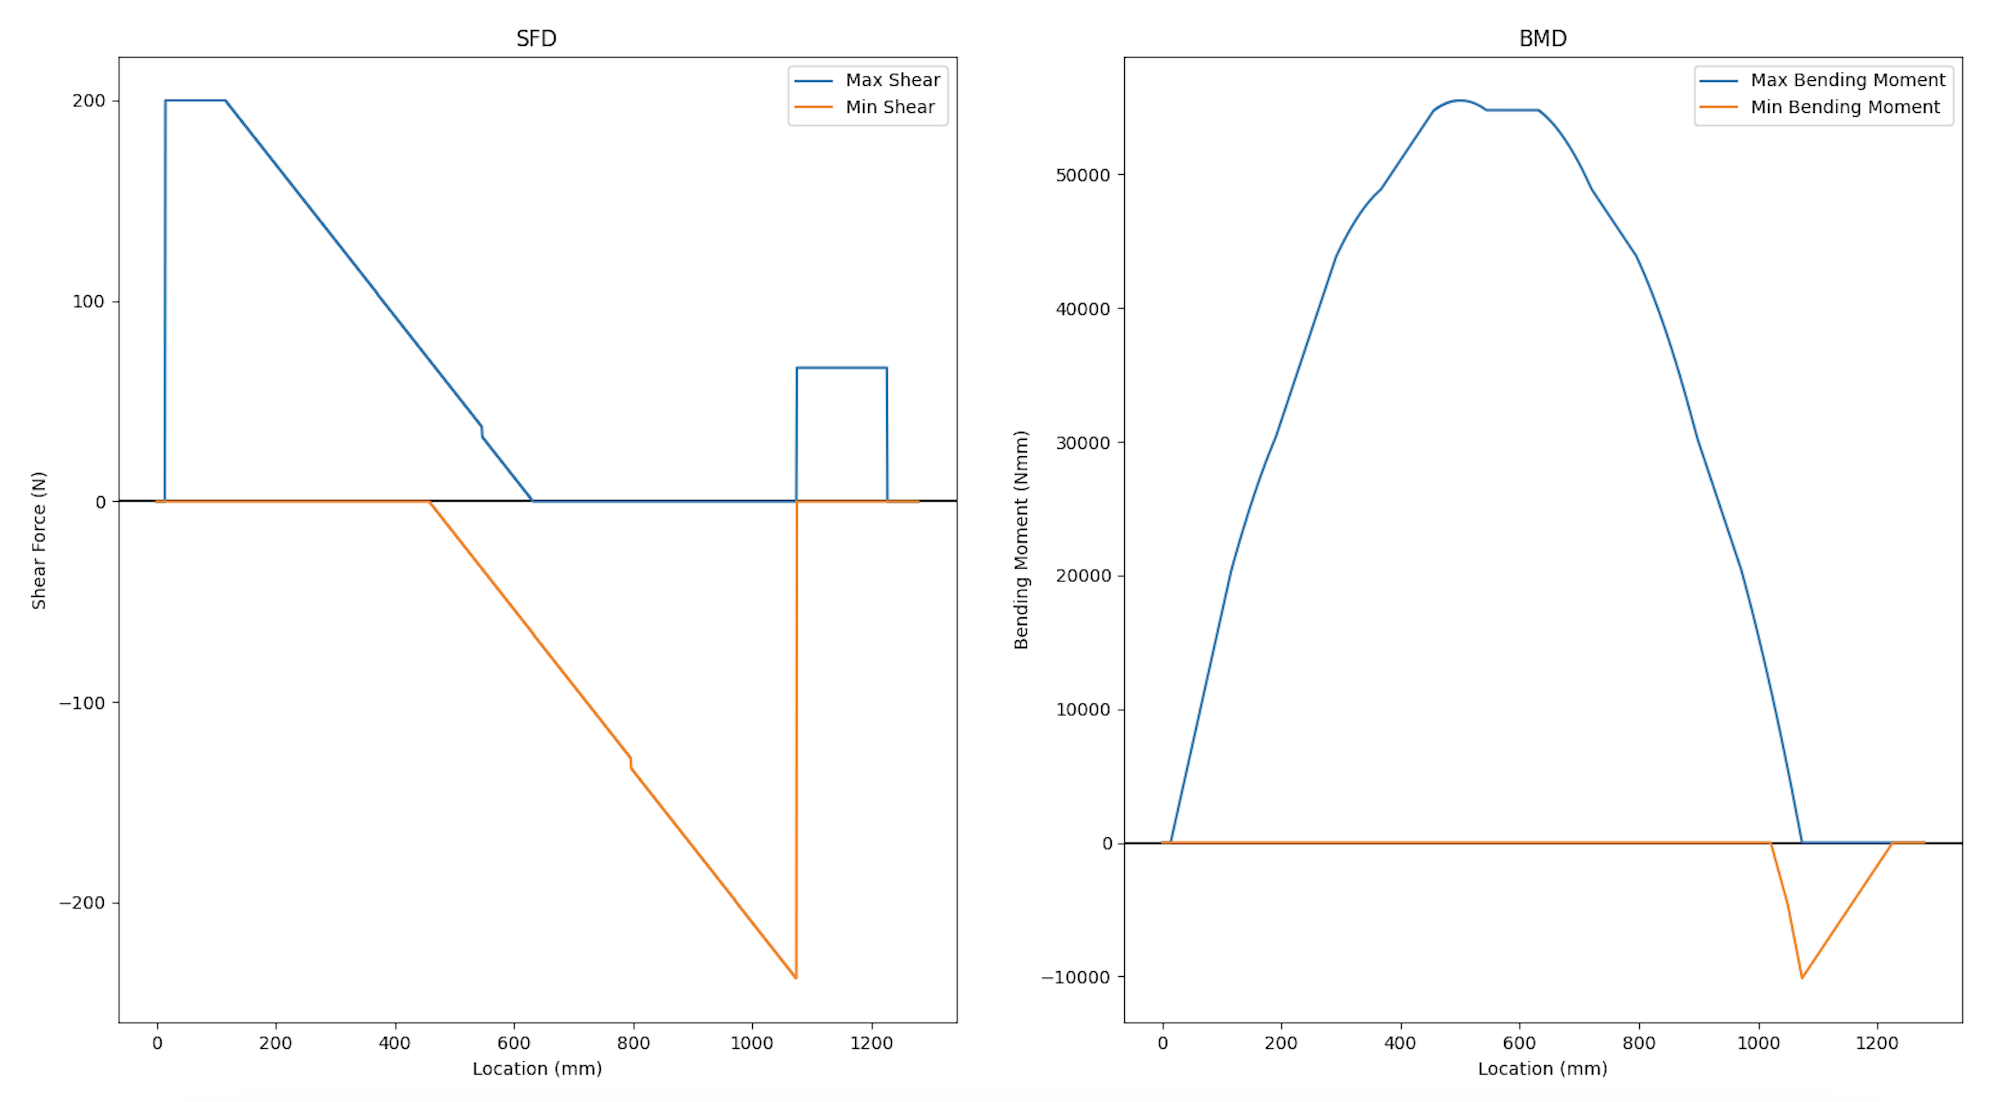
\includegraphics[width=.39\textwidth]{figures/SBTrainMaxDesign0.png}
    \caption {Envelope showing the maximum and minimum shear and bending moment across all train locations}
  \hfill
\end{figure}
\subsection*{Point Load}
The bridge fails by two edge buckling at $P = 187.1\si{N}$. Without failure, midspan deflection at $P = 200\si{N}$ is $1.371\si{mm}$.
\begin{table}[h]
\begin{center}
\begin{tabular}{|cc|} 
\hline
\multicolumn{1}{|c}{FOS} & \multicolumn{1}{c|}{Value} \\
\hline
Shear &   $3.32$ \\
Bending Moment &   $0.934$ \\
\hline
\end{tabular}
\caption{Factor of Safety}
\end{center}
\end{table}


\begin{figure}[h!]
  \centering
    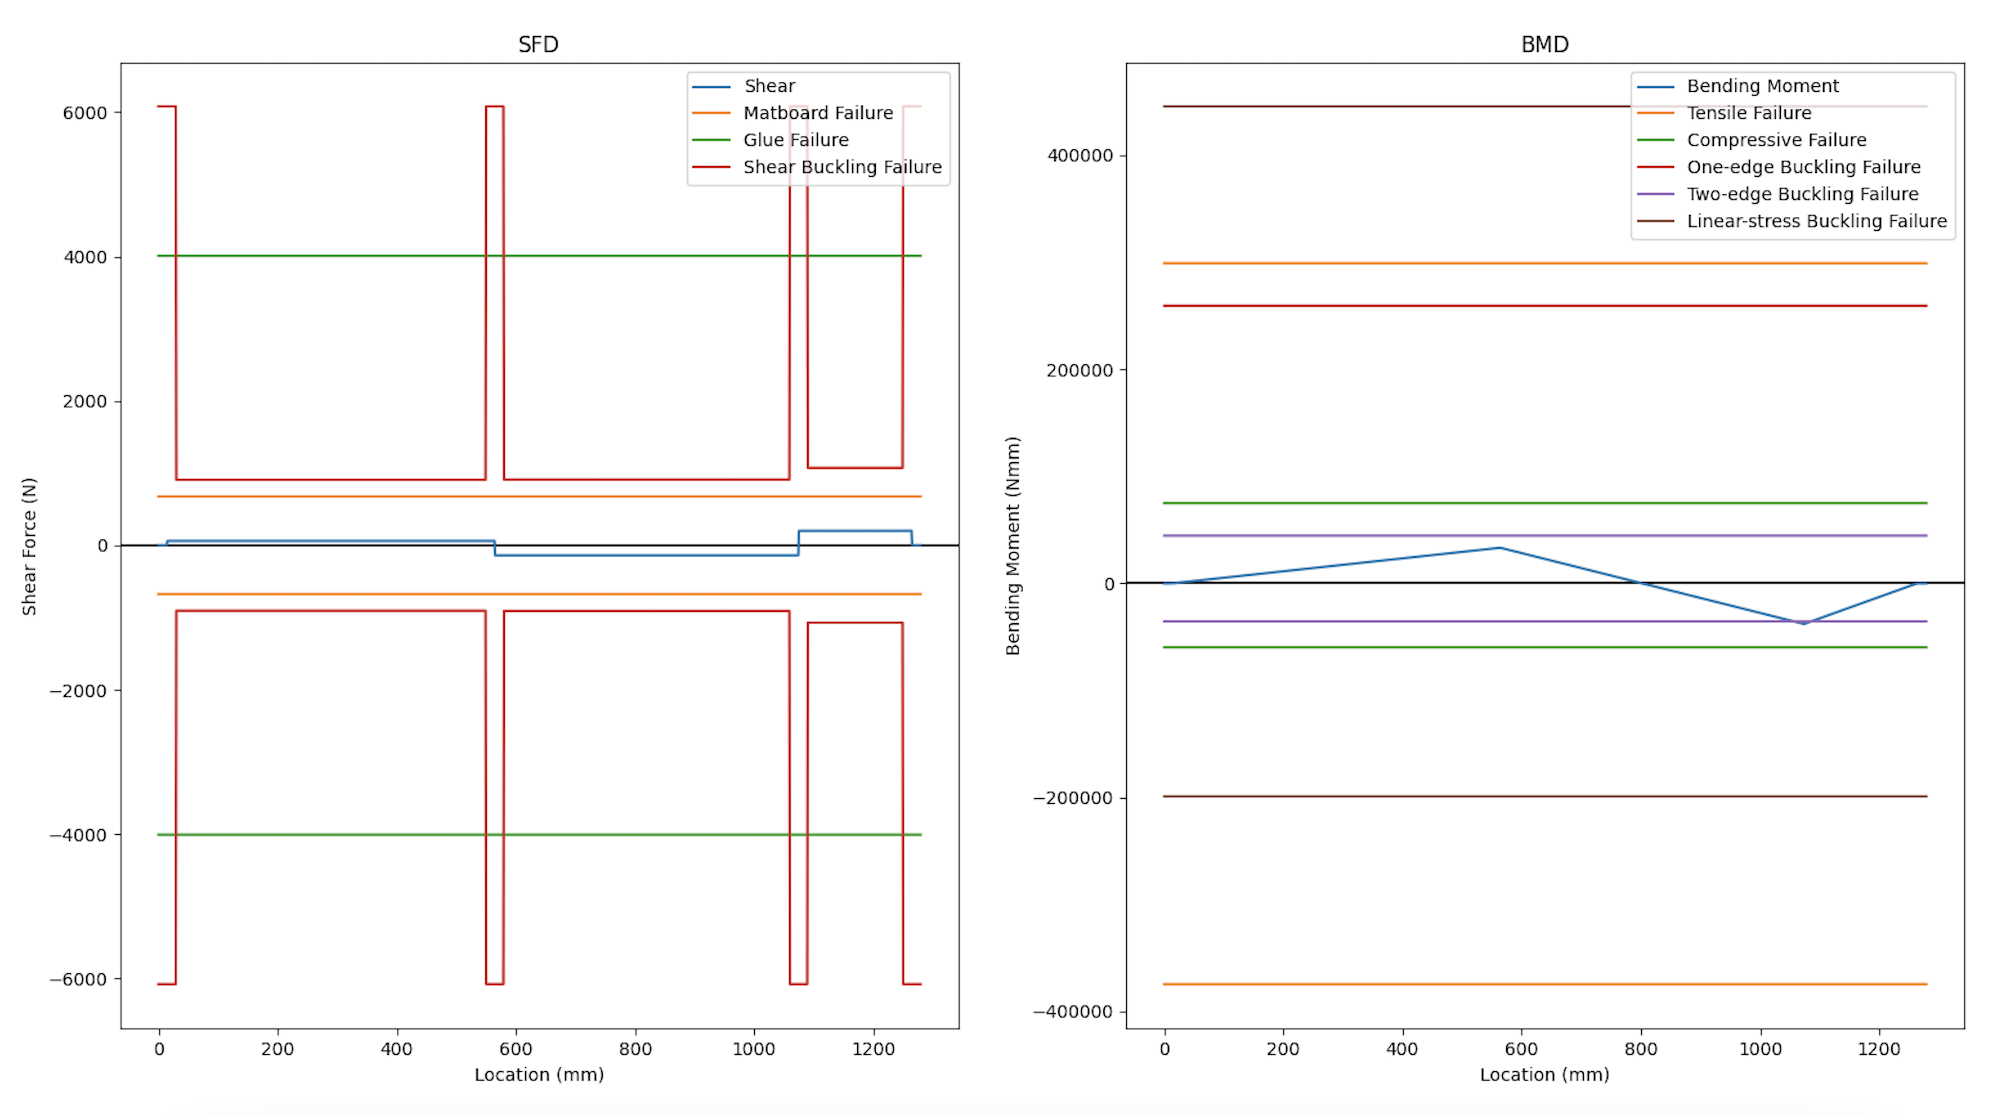
\includegraphics[width=.38\textwidth]{figures/SBPointDesign0.png}
    \caption {Point Loads of 200N (Design 0)}
  \hfill
\end{figure}


\begin{figure}[h!]
  \centering
    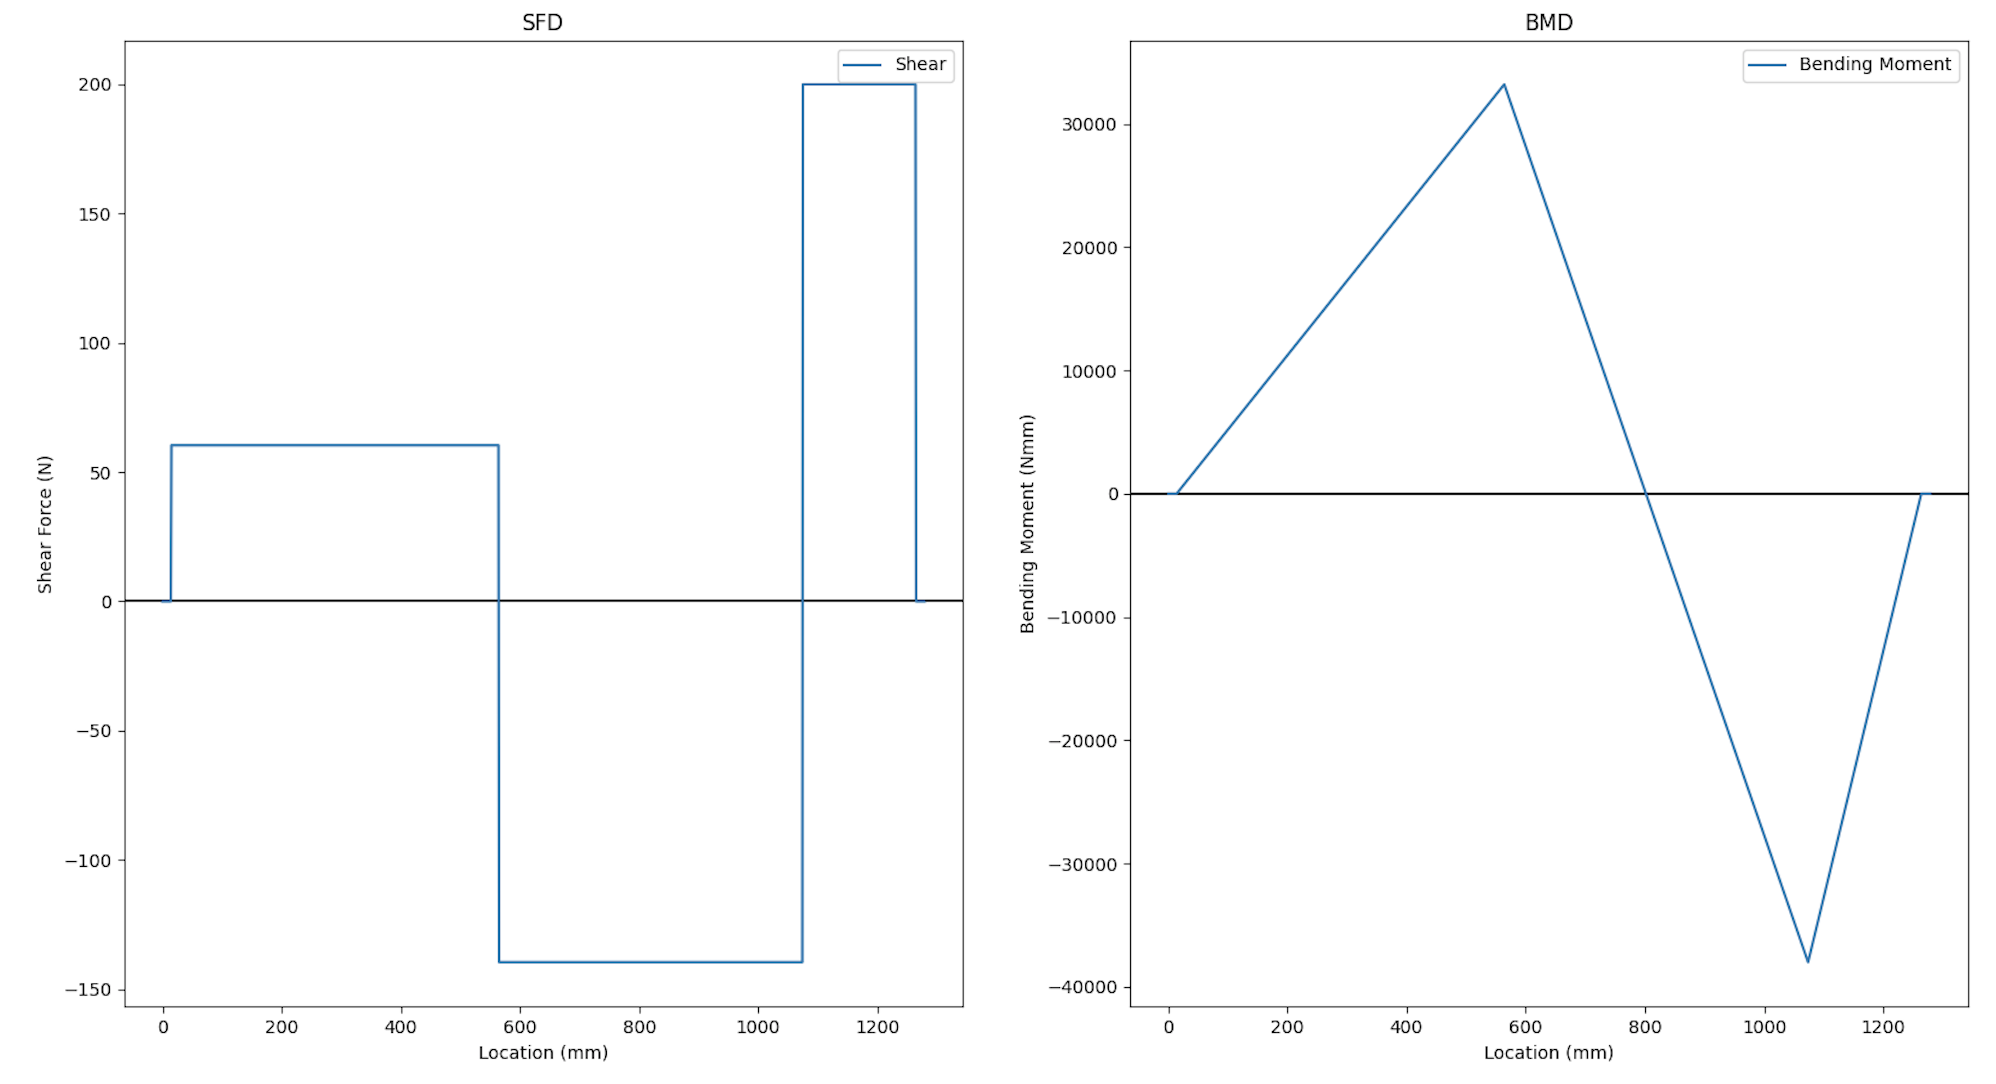
\includegraphics[width=.38\textwidth]{figures/CleanSBPointDesign0.png}
    \caption {Zoomed-in SFD and BMD for point loads of 200N}
  \hfill
\end{figure}

\section*{Final Design}

Detailed geometric properties of different cross sections can be found in drawings. 
\begin{figure}[h!]
  \centering
    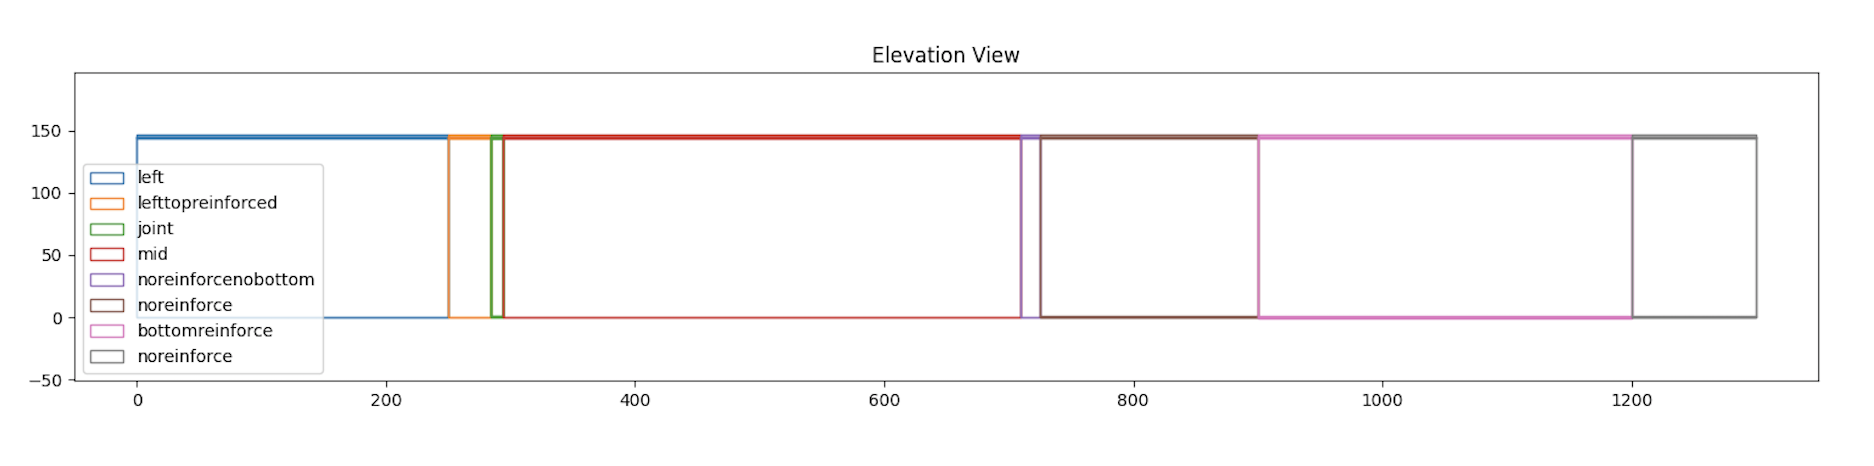
\includegraphics[width=.4\textwidth]{figures/elevationview.png}
    \vspace{1em}
    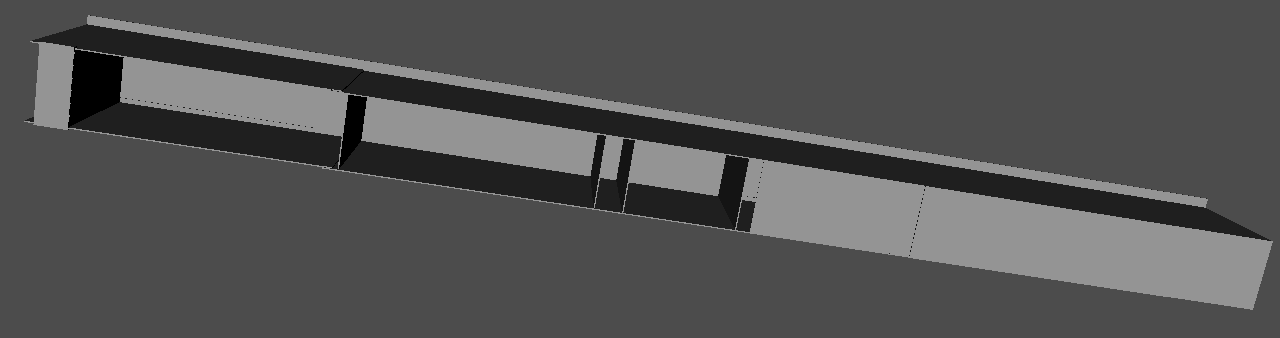
\includegraphics[width=.4\textwidth]{figures/3d bottom view.png}
    \caption {Elevation and 3D views of the Final Design}
  \hfill
\end{figure}


\subsection*{Train Load}
The final design survives the train load with a factor of safety of $2.45$ for shear and $1.554$ for bending moment.

\begin{table}[h]
\begin{center}
\begin{tabular}{|cc|} 
\hline
\multicolumn{1}{|c}{FOS} & \multicolumn{1}{c|}{Value} \\
\hline
Shear &   $2.45$ \\
Bending Moment &   $1.554$ \\
\hline
\end{tabular}
\caption{Factor of Safety}
\end{center}
\end{table}

\begin{figure}[h!]
  \centering
    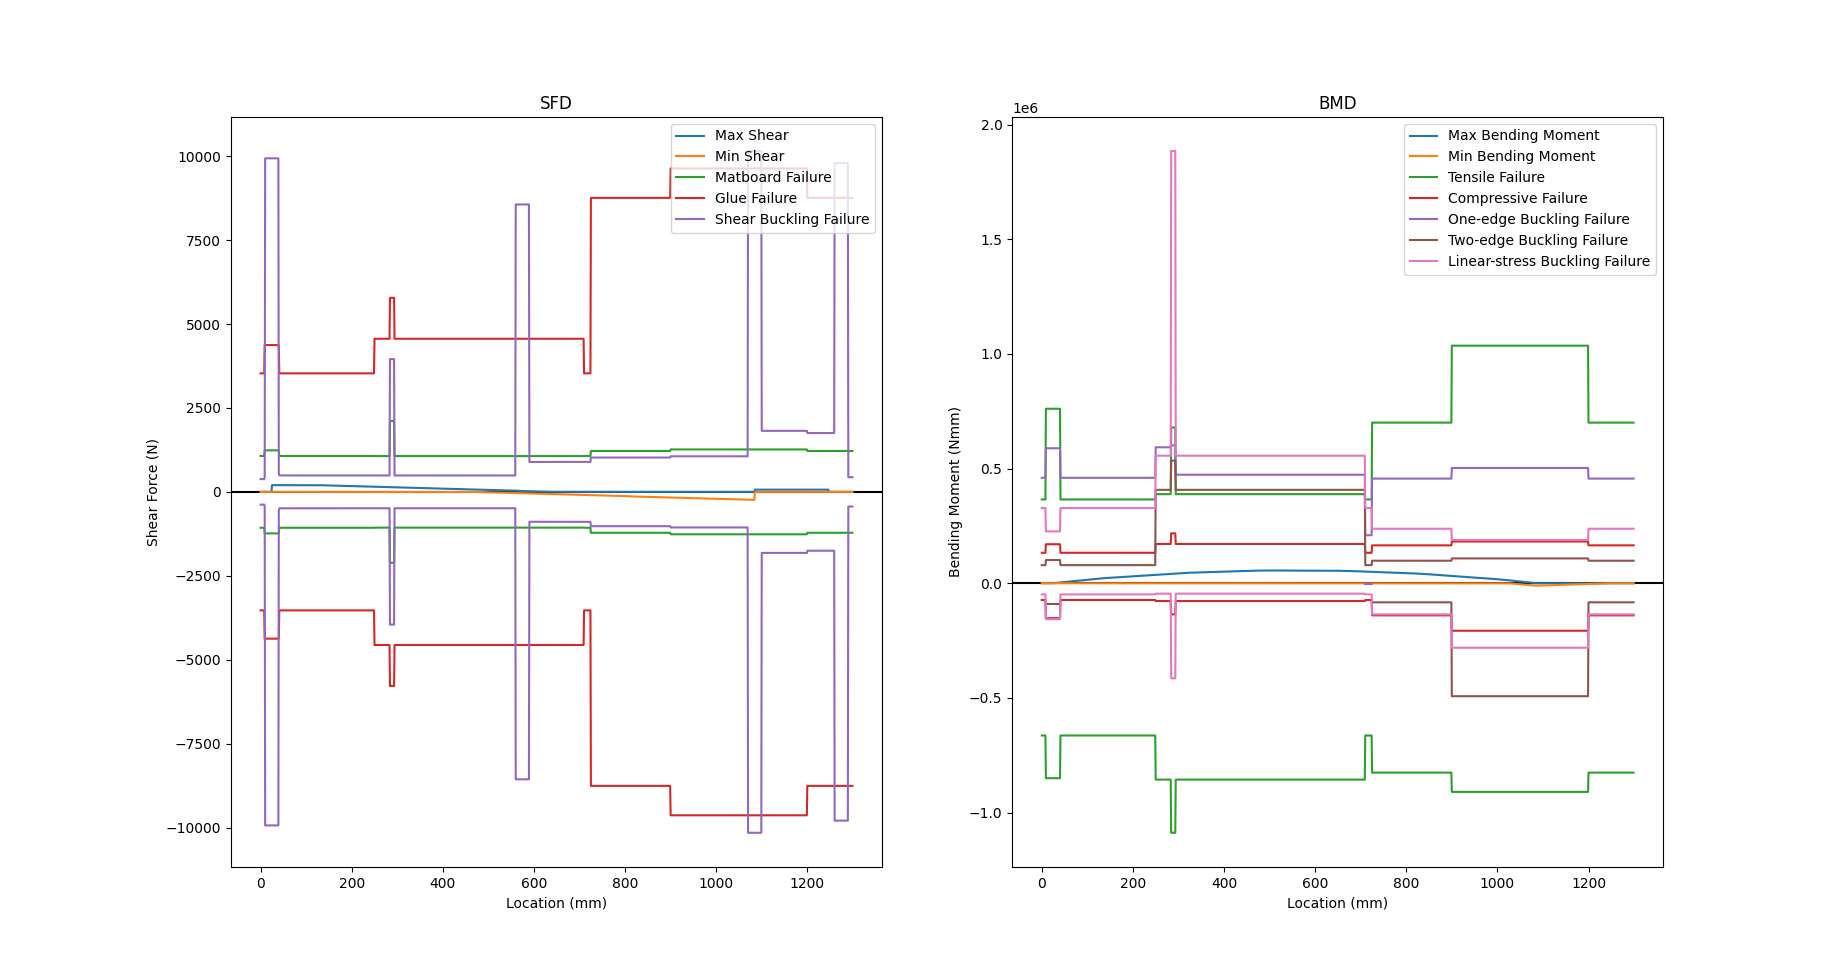
\includegraphics[width=.4\textwidth]{figures/SBTrainload.png}
    \caption {Train Load}
  \hfill
\end{figure}
\newpage
\subsection*{Point Load}
The bridge survives point loads of $200\si{N}$ and fails at $2064\si{N}$ in total by compression (crushing) of the top.
Midspan deflection under $P = 200$ is $0.470\si{mm}$.
\begin{table}[h]
\begin{center}
\begin{tabular}{|cc|} 
\hline
\multicolumn{1}{|c}{FOS} & \multicolumn{1}{c|}{Value} \\
\hline
Shear &   $6.09$ \\
Bending Moment &   $5.16$ \\
\hline
\end{tabular}
\caption{Factors of Safety for $200\si{N}$ point loads}
\end{center}
\end{table}

\begin{figure}[ht!]
  \centering
    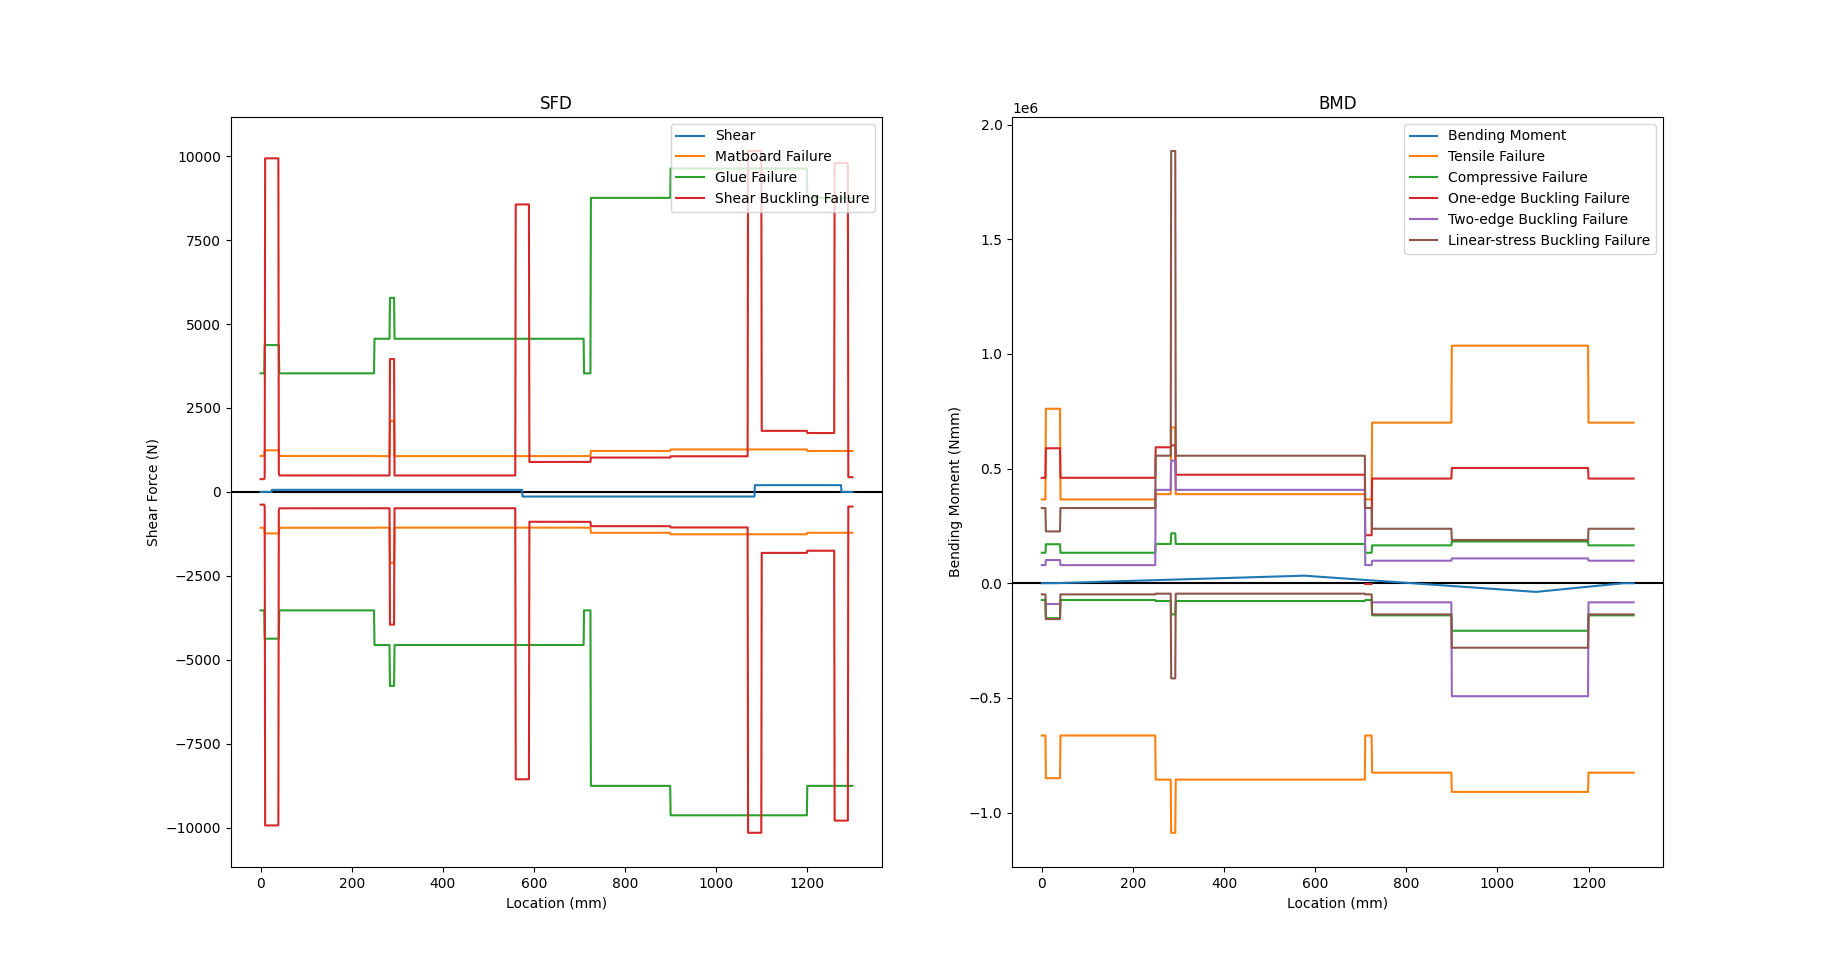
\includegraphics[width=.4\textwidth]{figures/SBPoint200.png}
    \caption {Point Load 200N}
  \hfill
\end{figure}

\begin{figure}[ht!]
  \centering
    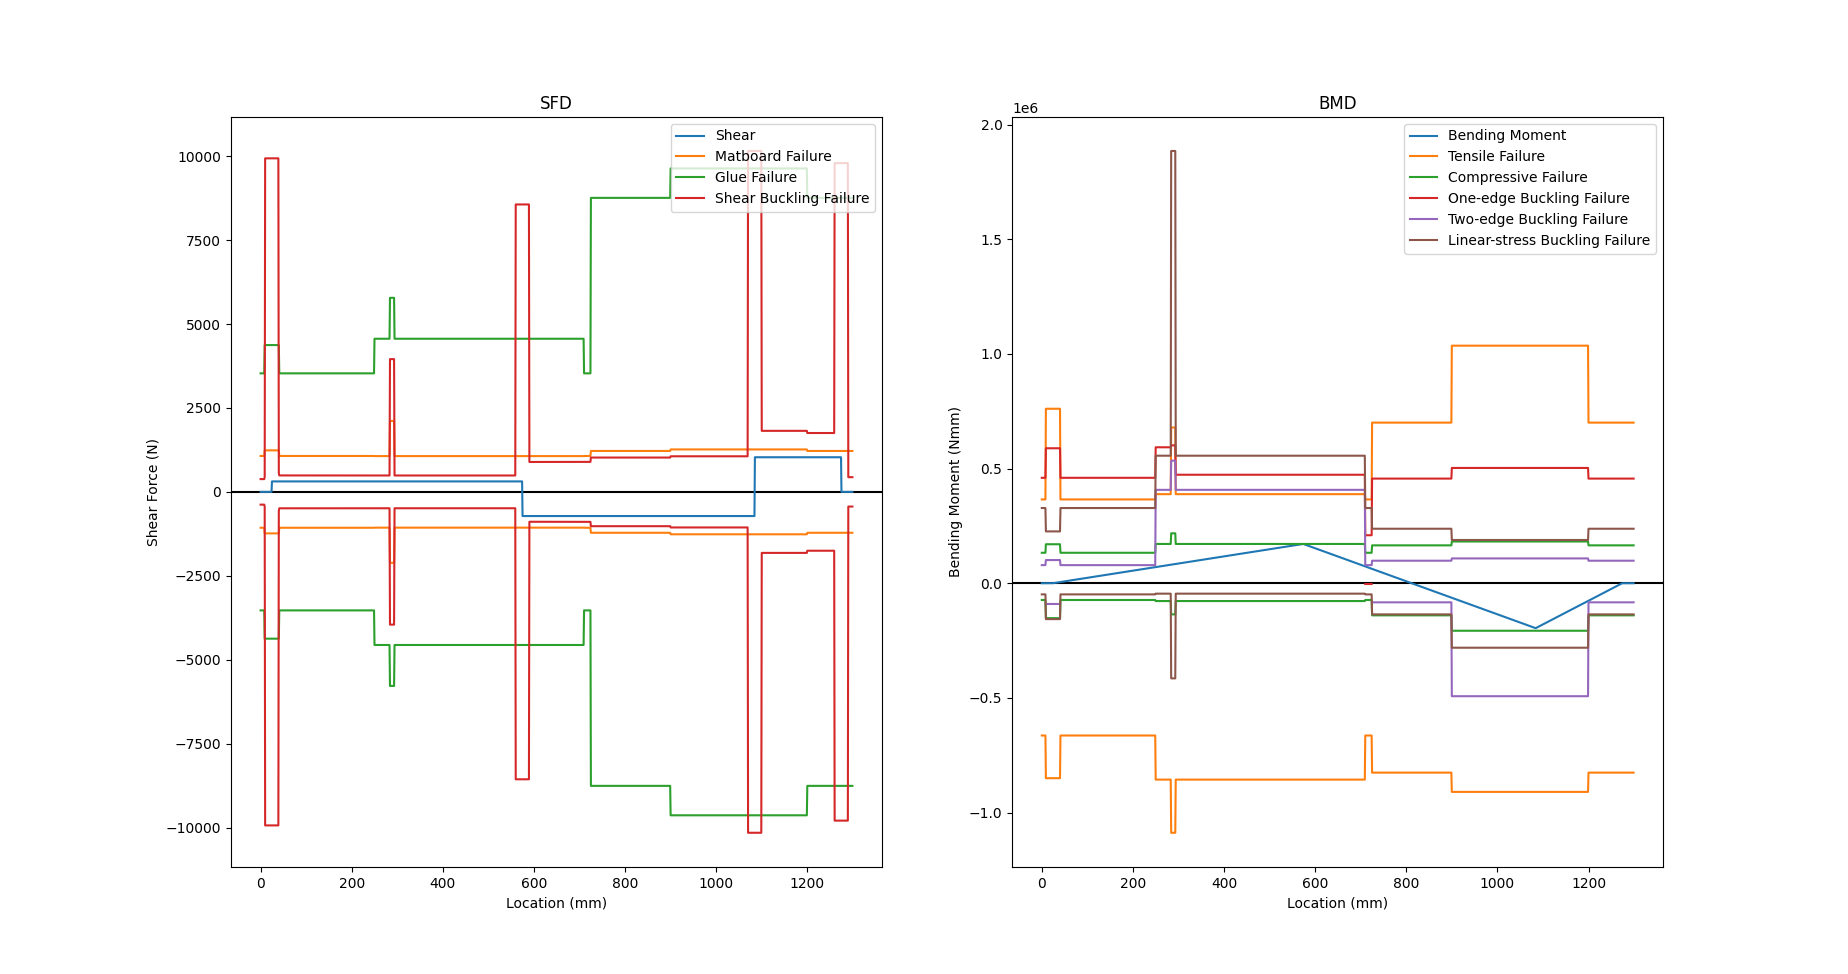
\includegraphics[width=.4\textwidth]{figures/SBPointFail.png}
    \caption {Compression Failure Point Load = 1032N}
  \hfill
\end{figure}

\section*{Improvements}
\begin{enumerate}
    \item Increase in the height of the bridge to prevent crushing
    \begin{itemize}
        \item $\sigma_{crit} = \frac{My}{I}$
        \item Increases both $I$ and $\Bar{y}$, however $I$ increases more since it goes up by the square, so $M$ increases and failure happens at a greater load.
    \end{itemize}
    \item Addition of top reinforcement and bottom reinforcement
    \begin{itemize}
        \item $\sigma_{crit} = \frac{4\pi^2E}{12-\mu^2}\left(\frac{t}{b}\right)^2 = \frac{My}{I}$
        \item Increases $I$, $\Bar{y}$ and thickness of the potential thin plate buckling area. $y$ will decrease from the shifting of $\Bar{y}$, $t$ will increase, and local buckling will happen at a greater load. 
    \end{itemize}
    \item Addition of joint
    \begin{itemize}
        \item Matboard is not long enough for a 1300mm bridge. The joint consists of a $1\si{cm}$ overlap of the walls glued together to resist shear, and reinforcements were later added to resist tension.
    \end{itemize}
    \item Addition of diaphragms
    \begin{itemize}
        \item $\tau_{crit} = \frac{5\pi^2E}{12(1-\mu^2)}\left[\left(\frac{t}{b}\right)^2+\left(\frac{t}{a}\right)^2\right] = \frac{VQ}{Ib}$
        \item Decreases $a$ for shear buckling, which is now a limiting factor due to the added height. 
    \end{itemize}
    \item Removal of bottom for certain parts of the bridge
    \begin{itemize}
        \item $\sigma_{crit} = \frac{My}{I}, \bar{y} = \sum A_id_i$
        \item Bending moment was determined to be always positive in that area, so no need to worry about buckling on the bottom. 
        \item In addition to saving material, this shifts $\Bar{y}$ up and decreases $y$ (distance between the top and the centroid) to reduce compression on the top. 
    \end{itemize}
    \item (Attempt at) reducing glue tab size 
    \begin{itemize}
        \item $\tau_{crit} = \frac{VQ}{Ib}$
        \item Saves material but reduces $b$ and failure shear force (shear failure will happen at a lighter load). But since the glue failure load is substantially higher than most other failure loads, this does not decrease the overall capacity.
        \item However, during construction it was observed that the smaller $5\si{mm}$ glue tabs are too hard to fold without damaging the material, so this decision was ultimately reverted.
    \end{itemize}
\end{enumerate}
    
\section*{Construction}
\begin{enumerate}
    \item Preparation (Figures \ref{fig:cutting_guide}, \ref{fig:cut_pieces})\\
    Before construction began, we organized the dimensions for all our pieces and obtained a cutting guide using \href{https://planetcalc.com/8634/}{an online tool}. Lines and labels were written on the matboard to indicate the lines of cutting and the uses of piece.\\ 
    Pieces were cut with a box cutter, and a ruler was used to ensure the pieces are cut straight.
    \begin{figure}[hbt!]
    \centering
        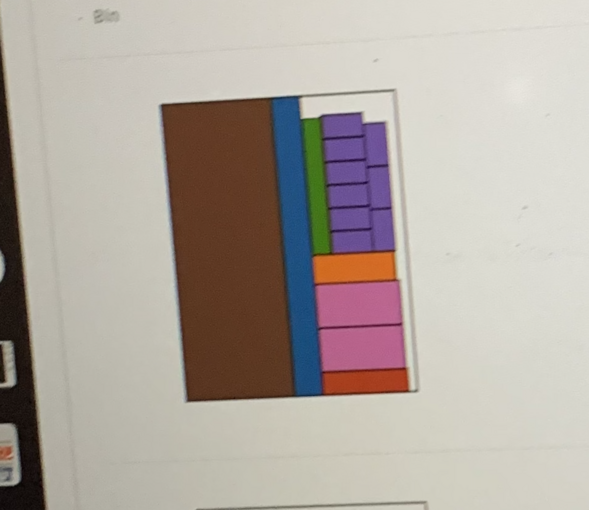
\includegraphics[width=.38\textwidth]{figures/prep1.png}
        \caption {Cutting Guide}
        \label{fig:cutting_guide}
    \hfill
    \end{figure}
    \begin{figure}[h!]
    \centering
        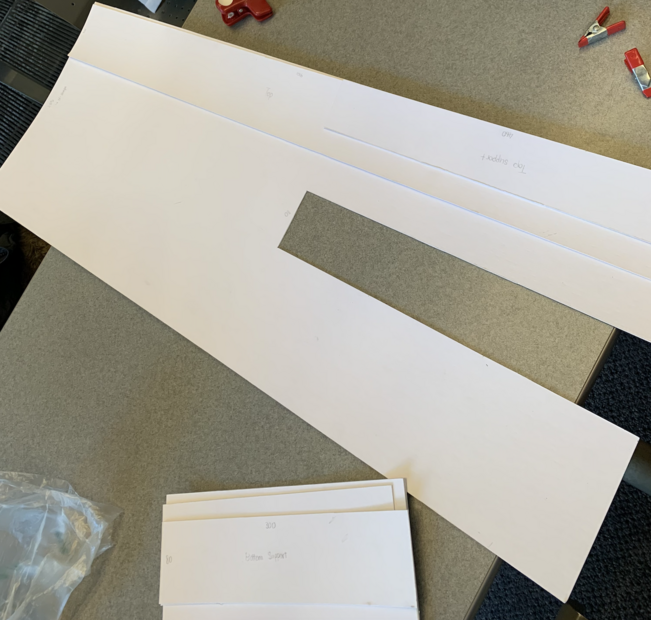
\includegraphics[width=.38\textwidth]{figures/prep2.png}
        \caption {Cut Pieces}
        \label{fig:cut_pieces}
    \hfill
    \end{figure}
    \item Scoring (Figure \ref{fig:scoring})\\
    In order to fold the matboard, the pieces were scored gently using a box cutter on the outside of the fold lines to prevent layer separation. The matboard was folded by aligning the ruler against the lines of scoring. This technique was applied to the main bridge body piece (U shape in Figure \ref{fig:cut_pieces}) and glue tabs.  
    \begin{figure}[h!]
    \centering
        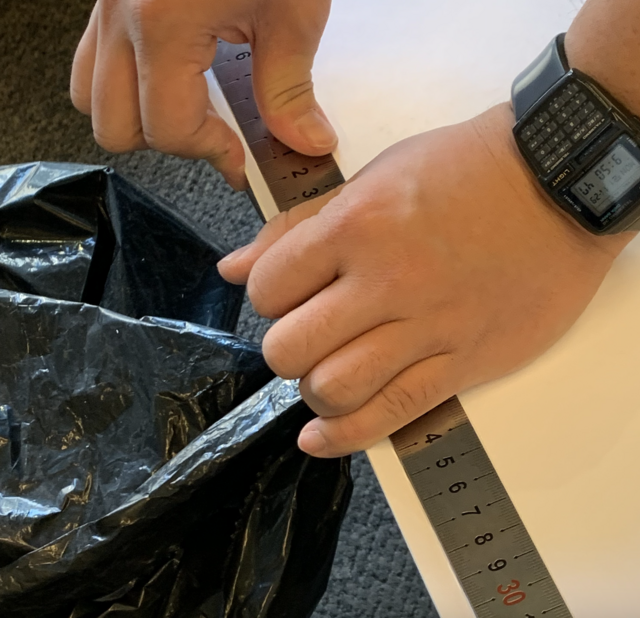
\includegraphics[width=.38\textwidth]{figures/scoring.png}
        \caption {Folding at scored locations}
        \label{fig:scoring}
    \hfill
    \end{figure}
    \item Adding Diaphragms (Figures \ref{fig:diaphragm1}, \ref{fig:diaphragm2})\\
    Locations of diaphragms were labeled on the main bridge body and glue was applied on the matboard.\\
    Glue was applied all sides of diaphragms. Diaphragms were attached to the glued main bridge body after dried. 
    \begin{figure}[h!]
    \centering
        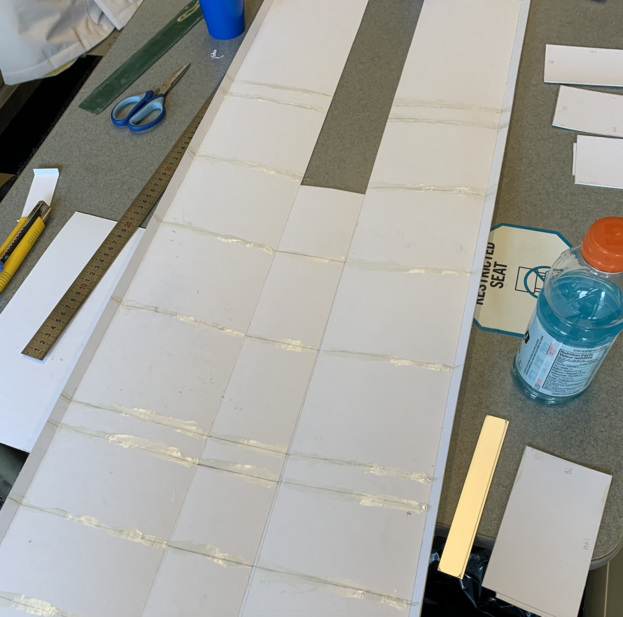
\includegraphics[width=.4\textwidth]{figures/adddia1.png}
        \caption {Glued Bridge Body}
        \label{fig:diaphragm1}
    \hfill
    \end{figure}
    \begin{figure}[h!]
    \centering
        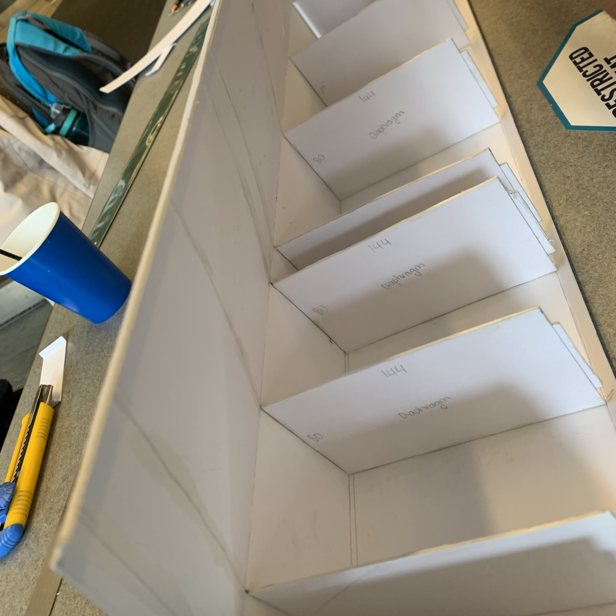
\includegraphics[width=.4\textwidth]{figures/add dia2.png}
        \caption {Attached Diaphragms}
        \label{fig:diaphragm2}
    \hfill
    \end{figure}
    \item Bridge Body (Figures \ref{fig:body1}, \ref{fig:body2})\\
    Bridge body was folded fully. Additional pieces at the circled location (Figure \ref{fig:body2}) were also attached to meet the length requirement. 
    \begin{figure}[h!]
    \centering
        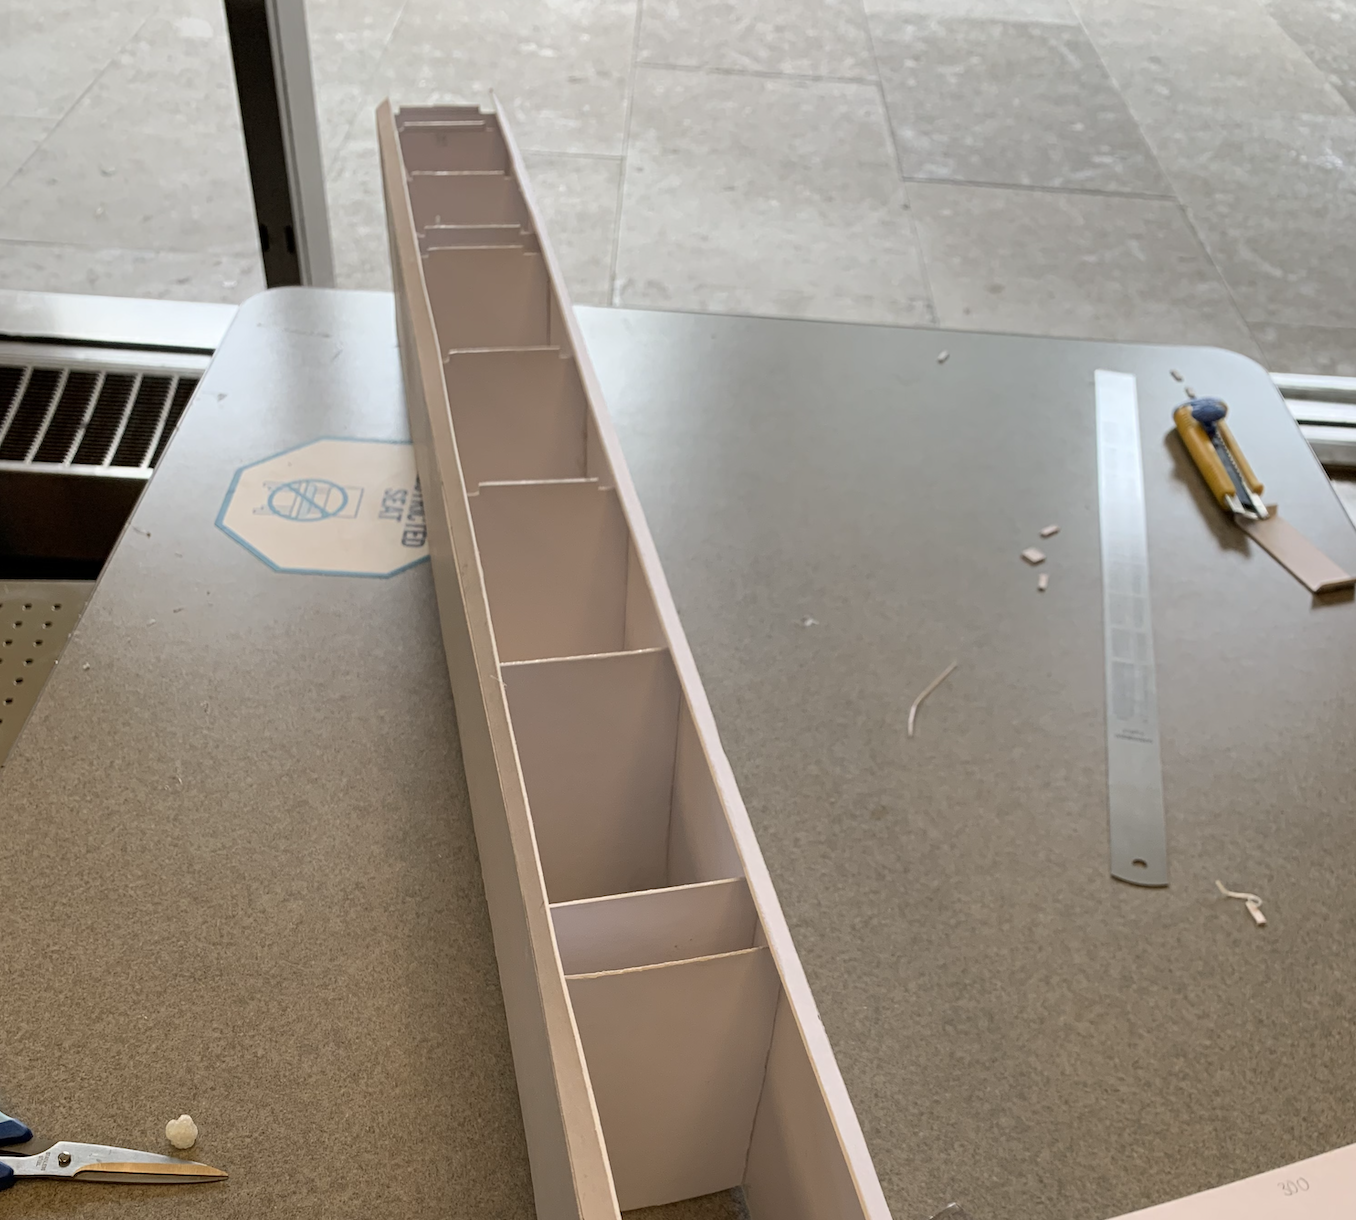
\includegraphics[width=.4\textwidth]{figures/bridgebody1.png}
        \caption {Folded Bridge Body}
        \label{fig:body1}
    \hfill
    \end{figure}
    \begin{figure}[h!]
    \centering
        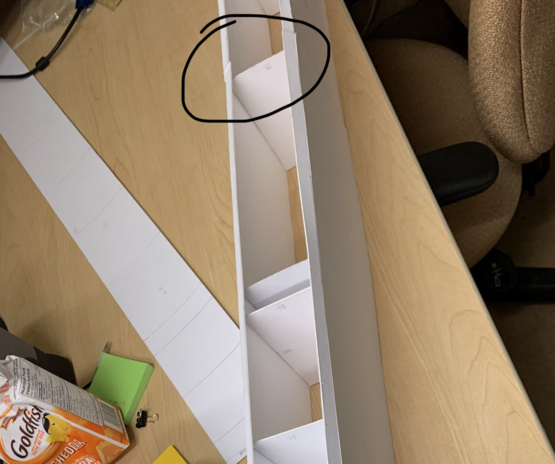
\includegraphics[width=.4\textwidth]{figures/bridge2.png}
        \caption {Lengthened Bridge Body}
        \label{fig:body2}
    \hfill
    \end{figure}
    \item Connecting Components to the Corresponding Glue Tabs (Figures \ref{fig:topreinforce}, \ref{fig:bottomreinforce})\\
    Top reinforcements were intended to be connected by sticking to the diaphragms. Locations of diaphragms were labeled using pencil and ruler. Then the top piece was attached to the bridge body by connecting with the glue tabs. \\
    Bottom reinforcement was attached to diaphragms at labeled locations. 
    \begin{figure}[h!]
    \centering
        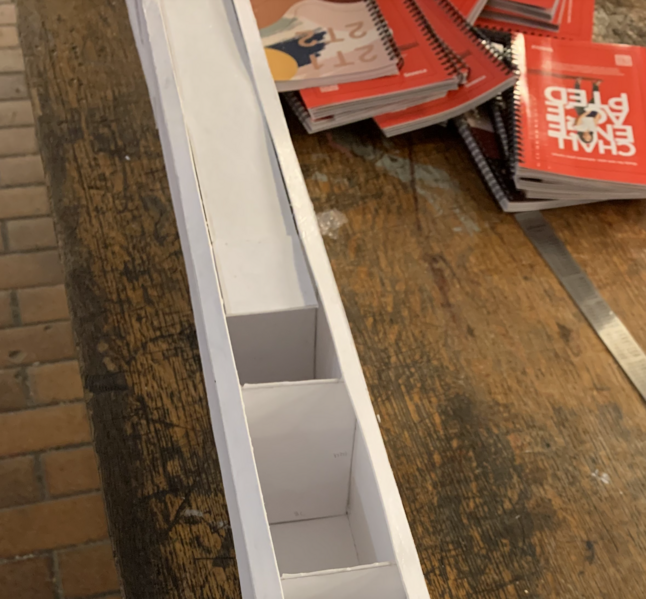
\includegraphics[width=.4\textwidth]{figures/toprein.png}
        \caption {Top Reinforcement}
        \label{fig:topreinforce}
    \hfill
    
    \end{figure}
    \begin{figure}[h!]
    \centering
        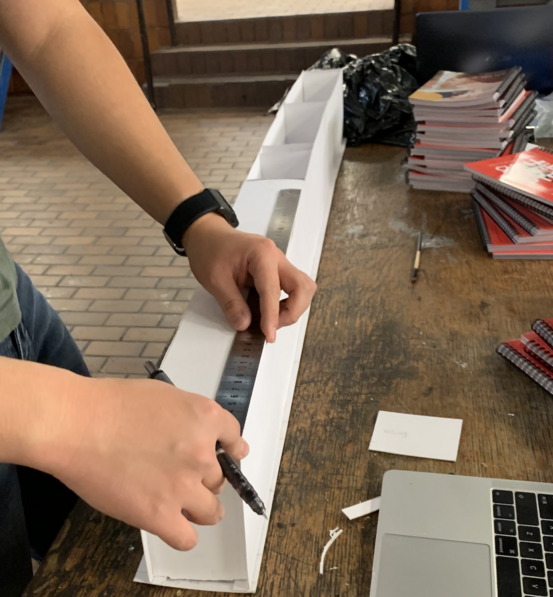
\includegraphics[width=.4\textwidth]{figures/bottomrein.png}
        \caption {Bottom Reinforcement}
        \label{fig:bottomreinforce}
    \hfill
    \end{figure}
    \newpage
    \item Setting (Figure \ref{fig:setting})\\
    After all the pieces are connected together, notebooks were placed on top of the bridge while setting the glue. Applying weights helped with setting the bridge into its ideal shape and keeping the glued areas in contact while the contact cement bonded.
    \begin{figure}[h!]
    \centering
        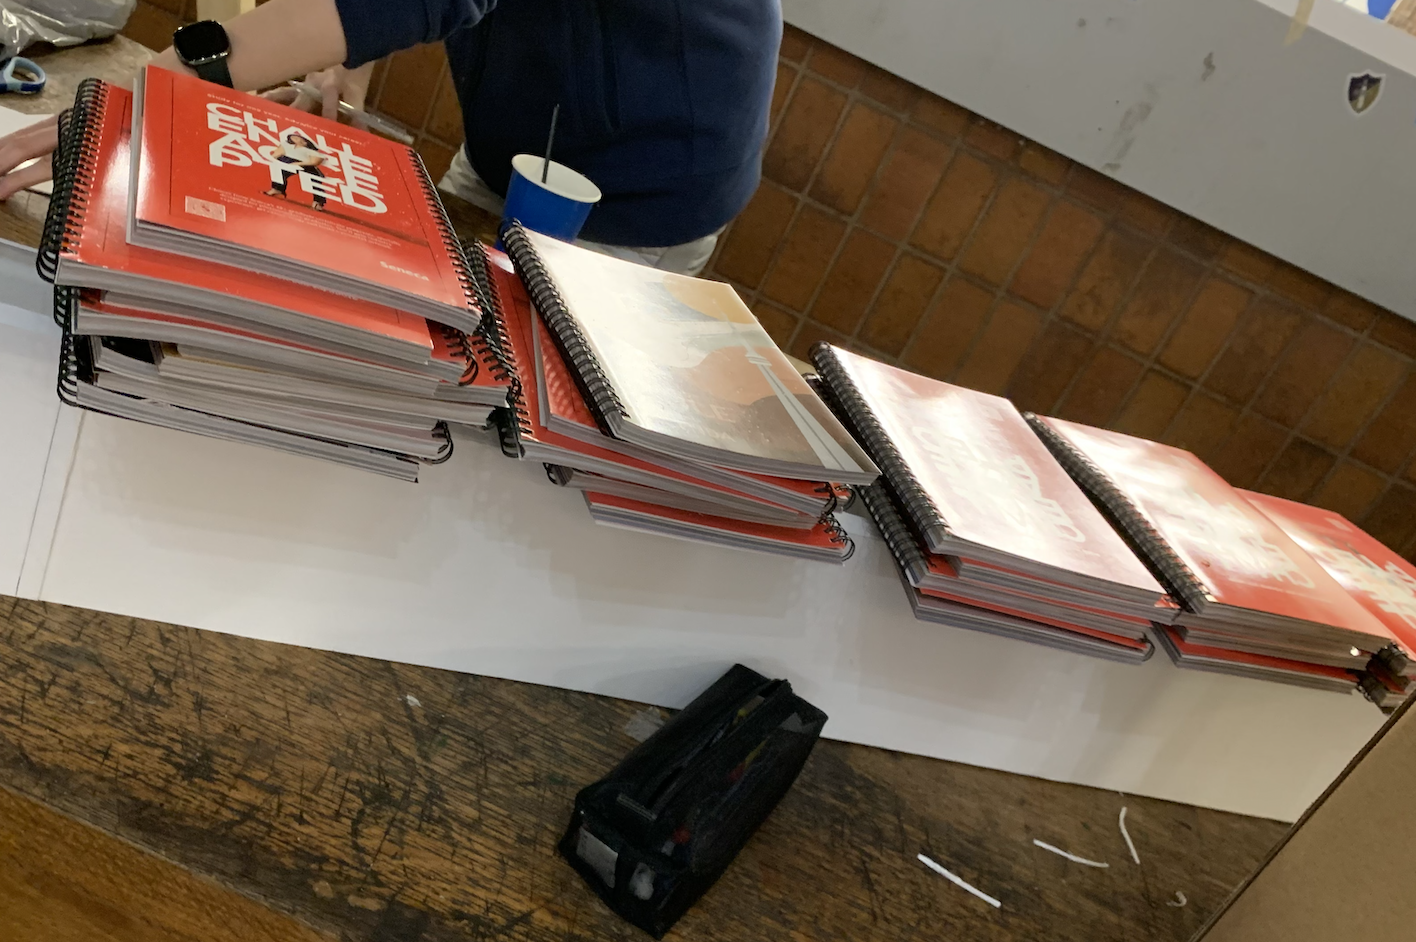
\includegraphics[width=.4\textwidth]{figures/settin.png}
        \caption {Setting Using Weights}
        \label{fig:setting}
    \hfill
    \end{figure}

\end{enumerate}
\section*{Deviation from Predicted Failure Load}
Assuming the code functioned properly, the theoretical predicted failure load is 2064N in total. However, due to construction errors and the limitations of the equations that were used in calculations, we predicted that the experimental failure load would be around 1000N. \\
\newline
\subsection*{Sources of Errors that Could Detract the Bridge Performance}
\begin{enumerate}
    \item When folding the matboard at some scored locations, there was shear between the layers of matboard, causing the layers to separate.
    \item There was one diaphragm that was placed slightly off, which required an additional piece of top reinforcement to cover it. 
    \item The internal width of the bridge was intended to be the same as width as the diaphragms. However, the bridge width appeared to be wider, causing vertical parts of the diaphragms failing to fully connect to the sides of the bridge. More glue was applied and additional pieces were added on the sides of the diaphragms to counteract this problem. 
    \item As the top of the matboard was slightly curved, the top parts of a few diaphragms failed to glue to the top of the bridge.
\end{enumerate}
\subsection*{Justification for the Newly Predicted Value}
\begin{enumerate}
    \item Most of our deviations comes from the diaphragms. The code predicted that in the worst case, if no diaphragms were effective, the bridge can hold about 850N in total.
    \item Teaching Assistants have informed us that most bridges can hold around 50\% of their predicted load.
\end{enumerate}
\section*{Workload Distribution}
Code: Tyler\\
Handwritten Calculations: Ivy, Julia\\
Report: Julia, Tyler\\
Engineering Drawings: Ivy\\
Bridge Optimization: Tyler, Ivy, Julia\\
\end{document}
